\documentclass[a4paper,ngerman,12pt]{scrartcl}

\usepackage[utf8]{inputenc}
%\usepackage[ansinew]{inputenc}

\usepackage[ngerman]{babel}

\usepackage{amsmath,amsthm,amssymb,stmaryrd,color,graphicx}
\usepackage{setspace}
\usepackage{bussproofs}
\usepackage{array}
\usepackage{comment}
\usepackage{wrapfig}

\usepackage{enumitem}

\usepackage{units}

\usepackage[protrusion=true,expansion=true]{microtype}

\usepackage{lmodern}

\usepackage{hyperref}
\usepackage{cleveref}

\newcommand{\RR}{\mathbb{R}}
\newcommand{\CC}{\mathbb{C}}
\newcommand{\ZZ}{\mathbb{Z}}
\newcommand{\NN}{\mathbb{N}}
\newcommand{\QQ}{\mathbb{Q}}

\setlength\parskip{\medskipamount}
\setlength\parindent{0pt}

\theoremstyle{definition}
\newtheorem{defn}{Definition}[]
\newtheorem{axiom}[defn]{Axiom}
\newtheorem{bsp}[defn]{Beispiel}

\theoremstyle{plain}
\newtheorem{prop}[defn]{Proposition}
\newtheorem{motto}[defn]{Motto}
\newtheorem{wunder}[defn]{Wunder}
\newtheorem{ueberlegung}[defn]{Überlegung}
\newtheorem{lemma}[defn]{Lemma}
\newtheorem{kor}[defn]{Korollar}
\newtheorem{hilfsaussage}[defn]{Hilfsaussage}
\newtheorem{satz}[defn]{Satz}
\newtheorem{frage}[defn]{Frage}

\theoremstyle{remark}
\newtheorem{bem}[defn]{Bemerkung}
\newtheorem{aufg}[defn]{Aufgabe}

\newtheorem*{antwort}{Antwort}

\newlength{\aufgabenskip}
\setlength{\aufgabenskip}{1.4em}
\newcounter{aufgabennummer}
\newenvironment{aufgabe}[1]{
	\addtocounter{aufgabennummer}{1}
	\textbf{Aufgabe \theaufgabennummer.} \emph{#1} \par
}{\vspace{\aufgabenskip}}

\clubpenalty=10000
\widowpenalty=10000
\displaywidowpenalty=10000

\setlength\unitlength{1cm}

\usepackage{tikz}

\RequirePackage{geometry}
\geometry{textwidth=16.0cm,textheight=24.5cm,footskip=1.5cm}

\begin{document}
	
\begin{picture}(0,0)
\put(0,-0.5){%
	
\includegraphics[scale=0.1]{logo-ifm}
}
\put(14.0,-3.5){%
	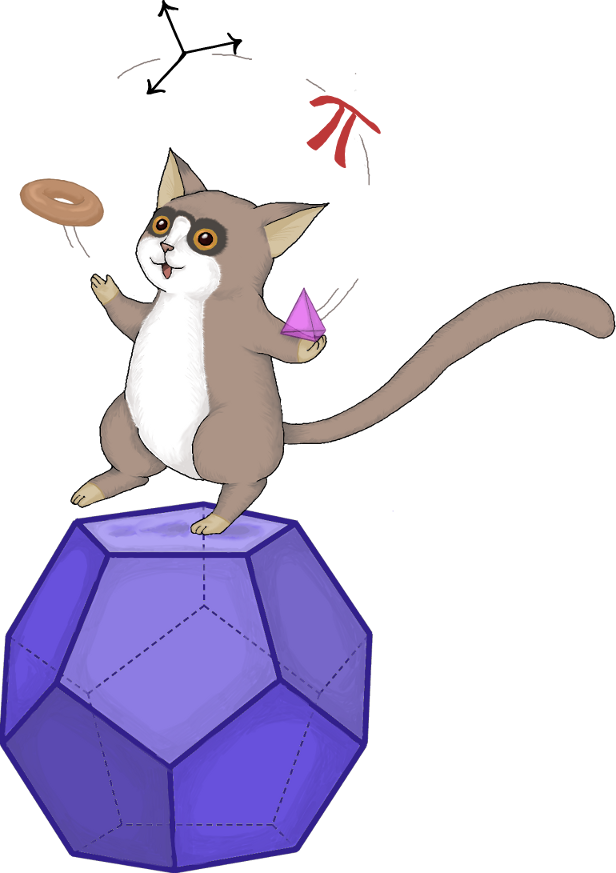
\includegraphics[scale=0.17]{cover}
}
\end{picture} 
	
\vspace{6em}

\section*{Unmöglichkeitsbeweise über Invarianten - Lösungshinweise}

Dieses Skript enthält Lösungs\emph{hinweise} zum letzten Korrespondenzbrief. Manchmal sind dies schon die kompletten Lösungen der Aufgaben, meistens sind es aber nur einige Hinweise, die dir dabei helfen sollen, auch die Aufgaben lösen zu können, bei denen du bisher nicht weiter gekommen bist. Wenn du noch weitere Fragen zu den Aufgaben hast, kannst du uns diese weiterhin gerne per E-Mail stellen.

Wenn du uns bereits deine eigenen Lösungsversuche geschickt hast (oder noch schicken wirst - das ist selbstverständlich immer noch möglich), dann versuchen wir natürlich auch dir mit unseren Korrekturen beim Verständnis der Aufgaben zu helfen. Es lohnt sich also uns deine Lösungen zu senden :-)

\begin{aufgabe}{}
	Das erste und das letzte Schachbrett lassen sich leicht nur mit roten 2x2-Tetrominos überdecken. Für das zweite und dritte Schachbrett ist das dagegen nicht möglich. Um dies zu beweisen kann man das folgende vierfarbige Schachbrett verwenden:

	\begin{center}
		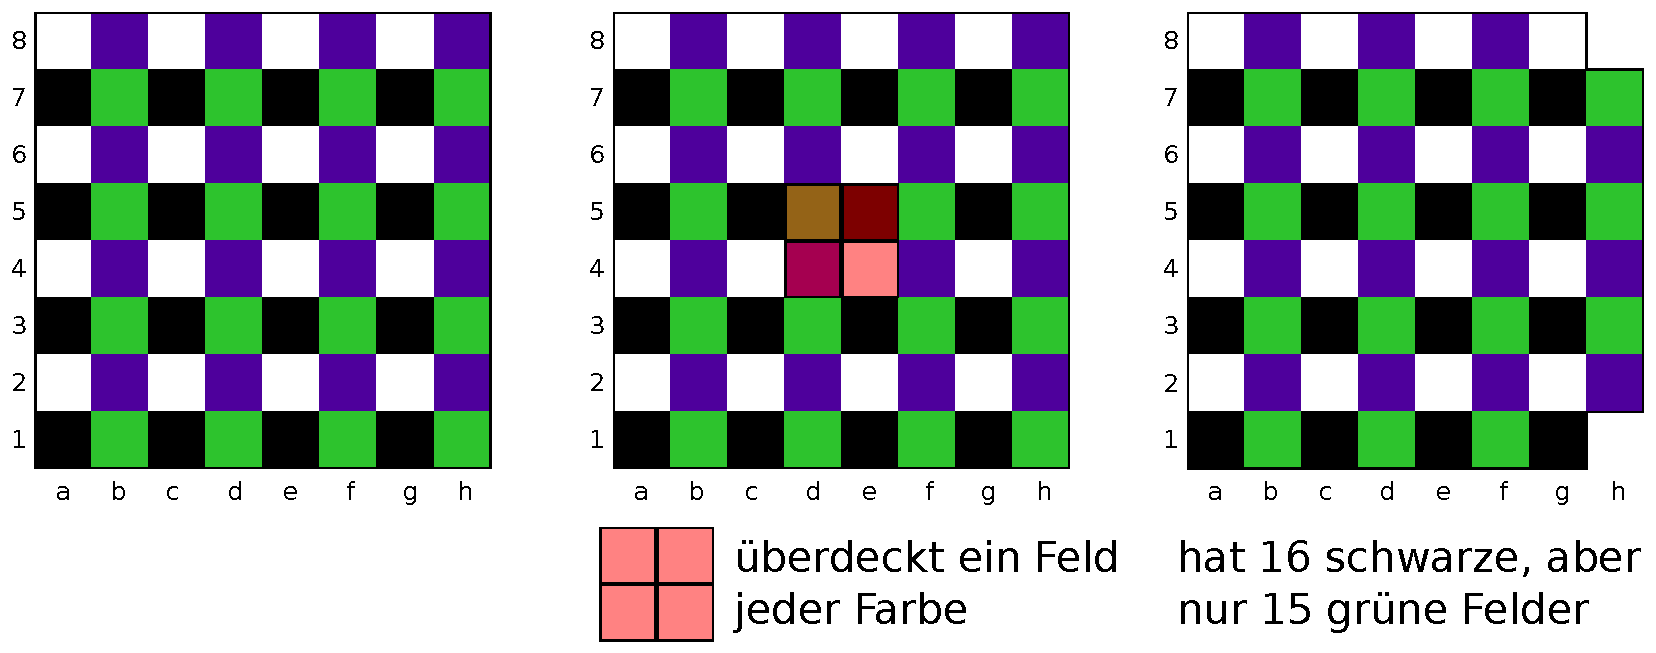
\includegraphics[width=.9\textwidth]{Bilder/Lsg-Aufgabe1.pdf}
	\end{center}
	
	Legt man einen 2x2-Tetrominostein auf dieses Brett, so bedeckt dieser immer genau ein Feld jeder der vier Farben. Möchte man das Brett nur mit solchen Steinen überdecken, muss es also von jeder Farbe gleich viele Felder haben. Sägt man jedoch wie bei den Schachbrettern 2 und 3 Felder heraus, ist dies nicht mehr der Fall (u.a. hat man in beiden Fällen mehr schwarze als grüne Felder übrig).
	
	Für das zweite Schachbrett gibt es auch noch einen einfacheren Beweis, dass es nicht mit 2x2-Steinen überdeckt werden kann. Jeder solche Stein bedeckt nämlich genau $4$ Felder, das zweite Schachbrett hat jedoch $62$ Felder - eine Zahl, die nicht durch $4$ teilbar ist.
\end{aufgabe}

\newpage
\begin{aufgabe}{}
	Das erste und dritte Schachbrett lassen sich mit 4x1-Tetromions überdecken. Das zweite und vierte dagegen nicht. Die Beweise dafür sind völlig analog zu Aufgabe 1, nur diesmal mit dem anderen vierfarbigen Schachbrett.
\end{aufgabe}

\begin{aufgabe}{Dreieckstetrominos}
	Die vier Dreieckstetrominos haben zusammen $16$ Felder und könnten daher theoretisch ein Dreieck aus $10$ schwarzen und $6$ weißen kleineren Dreiecken bilden (linkes Bild):
	\begin{center}
		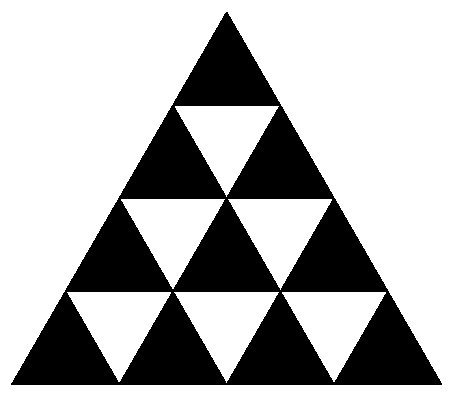
\includegraphics[width=.2\textwidth]{Bilder/Lsg-Aufgabe3.pdf} \qquad\qquad
		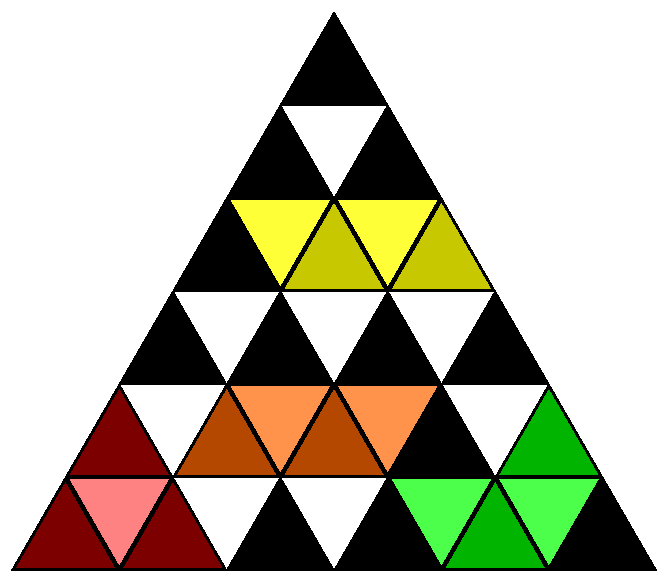
\includegraphics[width=.3\textwidth]{Bilder/Dreiecksschachbrett-Lsg.pdf}
	\end{center}	 
	Legt man nun die Dreiecksdominos auf ein solches Dreiecksmuster (rechtes Bild), so sieht man, dass drei der Steine (orange, gelb und grün) immer gleich viele schwarze wie weiße Felder überdecken. Sobald man diese drei Steine gelegt hat bleiben also noch $10-3\cdot2=4$ schwarze und $6-3\cdot2$ weiße Dreiecke übrig. Der verbleibende rote Stein müsste nun also vier schwarze Dreiecke überdecken, was offenkundig nicht möglich ist.
\end{aufgabe}

\begin{aufgabe}{}
	Hierfür gibt es natürlich sehr viele mögliche Antworten. Eine Startsituation, aus der heraus man eine Gleichverteilung erreichen kann, ist bspw.: 4 gelbe, 4 blaue und 1 grünes Chamäleon. Hier genügt schon eine einzige Begegnung, nämlich zwischen einem gelben und einem blauen Chamäleon.
	
	\textbf{Beachte:} In der Startsituation ist $C = 4 - 1 = 3$ durch 3 teilbar (was ja auch so sein muss - sonst könnten wir wie im Brief beweisen, dass niemals gleich viele Chamäleons jeder Farbe da sein können).
	
	Startsituationen aus denen heraus nie eine Gleichverteilung der Farben erreicht werden kann, sind u.a. all diejenigen in denen die Differenz zwischen der Zahl der blauen und der der grünen Chamäleons nicht durch $3$ teilbar ist (das haben wir ja im Brief gezeigt). Ein mögliches Beispiel wäre $7$ blaue, $6$ grüne und $2$ gelbe Chamäleons.
	
	Es gibt aber auch noch Startsituationen, in denen diese Differenz zwar durch $3$ teilbar ist, aber trotzdem niemals eine Gleichverteilung erreicht werden kann. Z.B. $5$ blaue, $2$ grüne und $1$ gelbes Chamäleon (weil die Gesamtzahl nicht durch $3$ teilbar ist) oder $39$ blaue, $0$ grüne und $0$ gelbe Chamäleons (weil die Chamäleons hier niemals ihre Farbe wechseln können).
\end{aufgabe}

\newpage
\begin{aufgabe}{Chamäleonmünzen}
	Muss man immer zwei Münzen gleichzeitig umdrehen, ist es nicht möglich gleich viele Bild- wie Zahlmünzen zu erhalten. Dies kann man z.B. mit folgender Invariante zeigen: Zu Beginn ist die Anzahl der Bildmünzen durch $2$ teilbar. Außerdem kann man sich leicht überlegen, dass jeder der drei möglichen Schritte nichts an dieser Invariante ändert. Also wird die Zahl der Bildmünzen immer durch $2$ teilbar sein. Um jedoch gleich viele Bild- wie Zahlmünzen zu haben, müsste man genau $3$ Bildmünzen erhalten - also eine \emph{nicht} durch $2$ teilbare Zahl. Folglich ist es nicht möglich diese Situation zu erreichen.
	
	Muss man immer genau drei Münzen umdrehen, kann man die gewünschte Situation sogar in nur einem einzigen Schritt erreichen:
	\begin{center}
		
\includegraphics[width=.5\textwidth]{Bilder/Lsg-Aufgabe5.pdf}
	\end{center}		
\end{aufgabe}

\begin{aufgabe}{}
	\begin{enumerate}
		\item Muss man pro Spielzug genau zwei Münzen umdrehen, ist es nicht möglich. Der Beweis dafür funktioniert genauso wie in Aufgabe 5, nur dass diesmal die Invariante \glqq Anzahl der Bildmünzen ist \emph{nicht} durch $3$ teilbar\grqq{} lautet.
		\item Muss man pro Spielzug genau drei Münzen umdrehen, ist es wieder ganz leicht möglich.
		\item Muss man pro Spielzug genau vier Münzen umdrehen, ist es nicht möglich. Der Beweis geht mit der gleichen Invariante wie im 1. Fall, nur dass es hier mehr mögliche Schritte gibt, für die man nachprüfen muss, ob die Invariante erhalten bleibt.
	\end{enumerate}
\end{aufgabe}

\begin{aufgabe}{}
Nur $2$er zu erhalten ist nicht möglich. Dies kannst du mit folgender Invariante zeigen: Zu Beginn ist die Summe aller Zahlen 
\[1+2+3+ \dots + 8 = 36\]
Wie man leicht sehen kann, ändert sich diese Summe nicht, wenn man einen Spielzug macht. Sie ist also tatsächlich eine Invariante.

Hätten wir irgendwann nur noch $2$er, so gäbe das aber eine Gesamtsumme von $8\cdot 2 = 16$ - also eine andere Zahl als die zu Beginn. Damit wissen wir, dass wir nie eine Spielsituation mit lauter $2$ern erreichen können.

Mit der gleichen Invariante lässt sich auch die Zusatzfrage beantworten (lässt sich $36$ durch $8$ teilen?).

\end{aufgabe}

\begin{aufgabe}{}
Nur $2$er zu erhalten ist unmöglich, wie man durch folgende Überlegung sehen kann. Als Invariante verwenden wir dazu die Aussage: \glqq Es gibt eine Zahl die größer oder gleich $8$ ist.\grqq

Zu Beginn ist diese Aussage offenbar wahr. Ist die Aussage nun vor einem Schritt wahr, wobei $m$ eine solche Zahl $\geq 8$ ist, so gibt es zwei Fälle zu unterscheiden:
\begin{enumerate}
	\item Wir verwenden die Zahl $m$ in diesem Schritt nicht. Dann ist sie nach dem Schritt immer noch da und folglich ist die Invariante weiterhin wahr. 
	\item Wir verwenden die Zahl $m$ zusammen mit einer weiteren Zahl $x$. Nach dem Schritt ist $m$ also nicht mehr da - dafür gibt es jetzt aber die Zahlen $m+x$ und $m-x$, wobei eine der beiden sicher größer als $m$ und damit auch größer als $8$ ist. Also ist die Invariante wiederum erfüllt.
\end{enumerate}
Wir haben also tatsächlich eine echte Invariante gefunden. 

In der Spielsituation aus lauter $2$ern ist nun aber keine Zahl mehr größer oder gleich $8$, d.h. diese Spielsituation erfüllt die Invariante nicht. Damit wissen wir, dass wir diese Situation niemals erreichen können.

Mit diesem Beweis haben wir übrigens auch automatisch schon gezeigt, dass es nicht möglich ist lauter $1$er, $3er$, \dots oder $7$er zu erhalten. Die kleinste Zahl, von der wir lauter gleiche bekommen können, ist folglich die $8$ - und tatsächlich ist das auch möglich:
\begin{align*}
\mathbf{1} \quad\vert\quad 2 \quad\vert\quad 3 \quad\vert\quad 4 \quad\vert\quad 5 \quad\vert\quad 6 \quad\vert\quad \mathbf{7} \quad\vert\quad 8 \\
6 \quad\vert\quad \mathbf{2} \quad\vert\quad 3 \quad\vert\quad 4 \quad\vert\quad 5 \quad\vert\quad \mathbf{6} \quad\vert\quad 8 \quad\vert\quad 8 \\
6 \quad\vert\quad 4 \quad\vert\quad \mathbf{3} \quad\vert\quad 4 \quad\vert\quad \mathbf{5} \quad\vert\quad 8 \quad\vert\quad 8 \quad\vert\quad 8 \\
6 \quad\vert\quad \mathbf{4} \quad\vert\quad 2 \quad\vert\quad \mathbf{4} \quad\vert\quad 8 \quad\vert\quad 8 \quad\vert\quad 8 \quad\vert\quad 8 \\
\mathbf{6} \quad\vert\quad 0 \quad\vert\quad \mathbf{2} \quad\vert\quad 8 \quad\vert\quad 8 \quad\vert\quad 8 \quad\vert\quad 8 \quad\vert\quad 8 \\
8 \quad\vert\quad \mathbf{0} \quad\vert\quad \mathbf{4} \quad\vert\quad 8 \quad\vert\quad 8 \quad\vert\quad 8 \quad\vert\quad 8 \quad\vert\quad 8 \\
8 \quad\vert\quad \mathbf{4} \quad\vert\quad \mathbf{4} \quad\vert\quad 8 \quad\vert\quad 8 \quad\vert\quad 8 \quad\vert\quad 8 \quad\vert\quad 8 \\
\mathbf{8} \quad\vert\quad \mathbf{0} \quad\vert\quad 8 \quad\vert\quad 8 \quad\vert\quad 8 \quad\vert\quad 8 \quad\vert\quad 8 \quad\vert\quad 8 \\
8 \quad\vert\quad 8 \quad\vert\quad 8 \quad\vert\quad 8 \quad\vert\quad 8 \quad\vert\quad 8 \quad\vert\quad 8 \quad\vert\quad 8
\end{align*}
\end{aufgabe}

\begin{aufgabe}{Produkte und Summen auf dem Schachbrett}
	Es ist nicht möglich. Um das auch zu beweisen betrachten wir zunächst drei Fälle, die in einem einzelnen Schritt auftreten können:
	\begin{enumerate}
		\item Beide gewählten Zahlen sind gerade: Dann ist auch Summe und Produkt dieser beiden Zahlen gerade - also ersetzen wir zwei gerade Zahlen durch zwei gerade Zahlen.
		\item Beide gewählte Zahlen sind ungerade: Dann ist deren Summe gerade und deren Produkt ungerade - also ersetzen wir zwei ungerade Zahlen durch eine ungerade und eine gerade Zahl
		\item Eine der gewählten Zahlen ist gerade und eine ungerade: Dann ist deren Summe ungerade und deren Produkt gerade - also ersetzen wir eine ungerade durch eine ungerade und eine gerade durch eine gerade Zahl.
	\end{enumerate}
	Insgesamt sehen wir also, dass die Anzahl der ungeraden Zahlen im ersten und dritten Fall gleich bleibt und im zweiten Fall um $1$ abnimmt. Wenn wir nun lauter gleiche Zahlen haben möchten, so müssen diese insbesondere entweder alle gerade oder alle ungerade sein. Da wir zu Beginn sowohl gerade als auch ungerade Zahlen haben und wir gerade Zahlen nicht loswerden können, bleibt als einzige Möglichkeit zu versuchen lauter (gleiche) gerade Zahlen zu bekommen.
	
	Angenommen das wäre möglich - dann müsste also die Anzahl der ungeraden Zahlen mit der Zeit immer weniger werden. Da wir pro Schritt höchstens eine ungerade Zahl loswerden können, muss es also insbesondere irgendwann einen Schritt geben, in dem wir nur noch eine einzige ungerade Zahl haben. Diese letzte ungerade Zahl können wir nun aber nicht mehr loswerden. Denn wenn wir in die Auflistung der verschiedenen Fälle oben schauen, sehen wir, dass wir nur dann eine ungerade Zahl los werden können, wenn wir in einem Schritt \emph{zwei} ungerade Zahlen auswählen. Da nun aber nur noch eine einzige ungerade Zahl übrig ist, ist das ab sofort nicht mehr möglich.
	
	Insgesamt können wir also niemals alle ungeraden Zahlen zu geraden Zahlen machen - und damit insbesondere niemals lauter gleiche Zahlen erhalten.
\end{aufgabe}

\end{document}